% !TEX root = Report.tex

\documentclass[12pt]{report}

\input usepackages
\input macros


\begin{document}
\beforepreface

\thispagestyle{empty}
\null\vfill
\begin{center}
%\textbf{Dedications}
%\linebreak
\textsl{Dedicated to my family and true friends.}
\end{center}
\vfill

\prefacesection{Abstract}
Automatic differentiation (AD) is a set of techniques to evaluate numerically the derivative of a function specified by a computer program. The FADBAD++ package developed by Ole Stauning and Claus Bendtsen implements the forward, backward, and Taylor modes utilizing C++ templates and operator overloading. 
It enables users to differentiate functions that are implemented in built-in C++ arithmetic types (such as double) or other customized class types. This report describes a multi-precision extension of the forward and Taylor modes in FADBAD++  using the GNU MPFR library.
\prefacesection{Acknowledgements}

 I would like to profusely thank Dr.\ Ned Nedialkov for his invaluable inculcation and great patience that helped me accomplish this project. I also want to show my appreciation to Gary Tan and Shawn Li, two honorable men who gave me a lot of help and encouragement during the project and in daily life. I would also like to show my gratitude to every professor, such as Dr.\ Franya Franek, Dr.\ George Karakostas, Dr.\ Ridha Khedri etc, in my graduation courses, who selflessly shared their knowledge and experience with me.
 
 

%\include{notation}
\afterpreface                      % command to create the parts of your thesis that come after your preface like contents and etc.

%\tableofcontents
\setcounter{figure}{0}
\setcounter{equation}{0}
\setcounter{table}{0}

% !TEX root = Report.tex

\chapter{Introduction}
Automatic differentiation (AD) is a set of techniques to evaluate numerically the derivative of a function specified by a computer program. AD exploits the fact that every computer program, no matter how complicated, executes a sequence of elementary arithmetic operations (addition, subtraction, multiplication, division) and elementary functions (exp, log, sin, cos, etc.) \cite{wikiAD}. By applying the chain rule repeatedly to these operations, derivatives of arbitrary order can be computed automatically, and accurately to the working precision \cite{Griewank2008}.

The \FADBADpp package developed by Ole Stauning and Claus Bendtsen implements the forward, backward, and Taylor modes utilizing \Cpp templates and overloaded operators. It enables users to differentiate functions that are implemented in built-in \Cpp arithmetic types (such as double) or other customized class types. The package consists of four files: \fadbad defines elementary functions inside, \fadiff defines a template \Fn to implement the forward mode, \badiff defines a template \Bn to implement the backward mode, and \tadiff defines a template \Tn  to implement the Taylor mode.

To extend to multiple precision the forward and Taylor modes in the original \FADBADpp package, we need a library capable of processing computation on multi-precision floating-point numbers. In our work, we use \MPFR (Multiple Precision Floating-Point Reliable Library), a portable library written in C for arbitrary precision arithmetic on floating-point numbers. However, the \FADBADpp package utilizes templates which require built-in \Cpp types or customized class types. Therefore we resort to \MPFRCpp, a wrapper for the \MPFR library that implements constructors, destructors, overloaded operators, and other \Cpp features.The class in the wrapper \MPFRCpp is named \mpreal. 

Many elementary functions in \fadbad, such as \texttt{mySin},  \texttt{myCos}, and \texttt{myExp},  use the corresponding functions  \texttt{sin},  \texttt{cos}, and \texttt{exp}, defined in \texttt{math.h}. However, these functions in the C numerics library {\tt math.h} only support built-in types in \Cpp such as float and double, but do not support \mpreal. Provided we have overloaded these elementary functions in the specialized operation struct in \fadbad, we could use the \mpreal class directly into the forward, backward, and Taylor series templates in the \FADBADpp package without doing any changes. But if we did that, there would be another deficiency: many temporary objects will be created from that. We will discuss the details in Chapter \CHref{extension}.

%all the overloaded operators functions defined in the \mpreal class return a class type \mpreal instead of a pointer or a reference, which means if we use the overloaded operators directly in the \FADBADpp package, it will create some temporary objects and it will be more a disaster if the overloaded operators is used in a nested loop.  To make the \FADBADpp package compatible with the \mpreal class, we need to modify the original \FADBADpp functions.

This report consists of four parts.
\begin{enumerate}
\item Summary of the \FADBADpp package
  
Chapter \CHref{summary} briefly introduces the mechanism of the \FADBADpp package, including the header file \fadbad, where universal elementary functions are defined, the header files \fadiff and \tadiff, where template classes for the forward and Taylor modes are defined.

\item Overview of \MPFR

Chapter \CHref{mpfr} gives an overview of the GNU \MPFR library to introduce how it can be used to deal with multi-precision computation. Furthermore, we will give an introduction to \MPFRCpp, a \Cpp wrapper for the \MPFR library.
 
\item Multi-precision extension in the \FADBADpp package
  
Chapter \CHref{extension} explains how to extend \FADBADpp to multiple precision. We will discuss issues about temporary objects construction if we use the \mpreal class directly in \FADBADpp templates. Then, we will show details regarding the extension step by step.
\item Examples
  
In Chapter \CHref{examples}, we will give several examples as a guide to show how to use the multi-precision feature in the modified \FADBADpp package.
\end{enumerate} 

%\renewcommand{\CHref}[1]{Chapter~\ref{ch:#1}}
%\TGN{
%\CHref{summary} briefly introduces \ldots

%\CHref{mpfr} gives an overview of the GNU \MPFR library. \ldots

%\CHref{extension} explains how to extend \FADBADpp to multiple precision. \ldots

%\CHref{examples} gives examples on how to use our modified \FADBADpp package. \ldots
%}

%\renewcommand{\CHref}[1]{\S\ref{ch:#1}}


% !TEX root = Report.tex

\chapter{Summary of \FADBADpp}\label{ch:summary}

We give a brief introduction to \FADBADpp in \SCref{introfadbad}. In \SCref{fadbad}, we introduce the static elementary functions and explain why it is necessary to specialize the struct and overload those functions for a user-defined data type. In \SCref{fadbadforwardmode}, we introduce the mechanism of the implementation of the forward mode in the FADBAD++ package and give a short example to explain how to use that template class. In \SCref{fadbadtaylormode}, we introduce the mechanism of the implementation of the Taylor mode in the FADBAD++ package and give a short example as well.

%\TGN{My scribbles above illustrate how to use the referencing macros. Need elaborate and rewrite. Also, write one such paragraph at the beginning of each chapter except the first.}

\section{Introduction}\label{sc:introfadbad}
The \FADBADpp package contains templates for performing automatic differentiation on functions implemented in C++ code. If the source code of a program, which is an implementation of a differentiable function, is available, then \FADBADpp can be applied to obtain the derivatives of this function \cite{FADBAD++}.

To apply automatic differentiation in a program, the arithmetic type used in the program  is changed to a customized type (\Fn, \B or \T). \F is the template class for the forward mode implementation, \B is the template class for the backward mode implementation, and \T is the template class for the Taylor mode implementation in the \FADBADpp package. 

\section{The fadbad.h file}\label{sc:fadbad}
The file \fadbad implements for a C++ typename {\tt T} a templated struct \Op that contains 29 static member functions. We call these 29 static member functions elementary functions in the following context.

We can call these functions outside the struct \Op to execute arithmetic operations for variables in C++ built-in types, such as float and double.
For example, {\tt Op<double>::myCadd(x,y)} executes {\tt x+=y} for a double type variable {\tt x} and a double type variable {\tt y}.

If {\tt T} is a built-in type, then all the elementary functions in \Op, such as {\tt mySin},  {\tt myCos}, and {\tt myExp}, call their corresponding functions {\tt sin},  {\tt cos}, and {\tt exp} in the C numerics library {\tt math.h}, which only supports C++ built-in types. 
For example, {\tt Op::mySin} is defined by

\texttt{static T mySin(const T \&x) \{ return ::sin(x); \}}

\noindent If {\tt x} is of type float or double, then {\tt Op<T>::mySin(x)}
%, defined by
%\texttt{static T mySin(const T \&x) \{ return ::sin(x); \}} \noindent in the struct \Op,
is equivalent to {\tt sin(x)}, where {\tt sin} is implemented in {\tt math.h}.

However, if {\tt T} is a user-defined data type, say {\tt Interval}, and an elementary function, like {\tt Op<Interval>::myExp}, is not specialized for {\tt Interval}, then it will go to the general template class \Op, and call the function {\tt Op<T>::myExp} inside. But, we cannot simply call {\tt Op<Interval>::myExp(x)} for a {\tt Interval} type variable {\tt x} because the corresponding arithmetic function {\tt exp} defined in {\tt math.h} does not support the type Interval. Similarly, since {\tt Op<Interval>::myExp} is called in the function {\tt fadbad::exp} for a data type {\tt F<Interval>} in the forward mode, as a chain effect, we cannot simply call {\tt fadbad::exp(xf)}, where xf is an {\tt F<Interval>} variable. In Chapter \CHref{extension}, we show how to specialize with the data type \mpreal to the general template class \Op. 

To inform the user about such specializations, \fadbad puts before the templated struct \Op the following message:

{\em The following template allows the user to change the operations that are used in \FADBADpp for computing the derivatives. This is useful as an example for specializing with non-standard types such as interval arithmetic types.}


\section{Forward Method}\label{sc:fadbadforwardmode}
The forward method of AD is implemented by a template class \Fn. An \F object contains a private member m\_val of \U type to store the value and an array of \U type to store the gradient of the variable. Following the chain rule repeatedly, the gradient array inside the result \F object will contain all the partial derivatives with respect to independent variables in the function.

There are two different versions of the \F template class. The version where the gradient array is allocated statically is called stack version, while the other one where the gradient array is allocated dynamically is called heap version. Since the mechanism and usage of these two versions are identical, we will just take the heap version for instance in this report.
\subsection{Overloaded elementary functions in \textbf\texttt{fadiff.h}}
The arithmetic operators and the elementary functions are overloaded in \fadiff. Here, as an example, we give the definition of the overloaded \texttt{sin} function.

%\TGN{This function looks overwhelming. Perhaps give the introductory example first, and then explain how this {\tt sin} works.}

\begin{lstlisting}[numbers=none]
template <typename T>
F<T> sin(const F<T>& a)
{
   F<T> c(Op<T>::mySin(a.val()));
   if (!a.depend())
   return c;
   T tmp(Op<T>::myCos(a.val()));
   c.setDepend(a);
   for (unsigned int i = 0; i < c.size(); ++i)
   c[ i ]            = a[ i ] * tmp;
   return c;
}
\end{lstlisting}

An \F object contains a value and a gradient. In those overloaded functions in \fadiff, the elementary operation functions such as \texttt{mySin},  \texttt{myCos}, and \texttt{myExp} in the \fadbad are called. For example, in the definition of the \texttt{sin} function above, static functions \texttt{mySin} and \texttt{myCos} are called to compute the value and the gradient array. Hence, by following the chain rule step by step, it will output a final result, an \F object with a value and a gradient of \U type inside \cite{IntroAD}. From the gradient array, all the partial derivatives could be obtained with respect to different variables.

\subsection{An introductory example of using the forward mode template class}
Suppose we have the function
\begin{equation}
f(x,y,z)=x+y\times\sin(z)
\label{eq:1}
\end{equation}
Then, we want to obtain partial derivatives with respect to $x$, $y$, and $z$, $df/dx$, $df/dy$, and $df/dz$. Now we are ready to differentiate this function by using the forward method template class \Fn.

If we work with doubles, all the input arguments should be of type \texttt{F<double>} as well as the returned variable.
\begin{lstlisting}[numbers=none]
F<double> func(const F<double>& x, const F<double>& y,  const F<double>& z)
{
	return x+y*sin(z);
}
\end{lstlisting}
Our function above is now prepared for computing derivatives. Before we call the function, we have to specify the variables we want to differentiate with respect to.  After the call, we obtain the function value and the derivatives stored in the object f. This can be done with the following code
\begin{lstlisting}[numbers=none]
F<double> x,y,z,f;   // Declare variables x,y,z,f
x=1;                 // Initialize variable x with value 1
x.diff(0,3);         // Set x as an independent variable of index 0 of 3
y=2;                 // Initialize variable y with value 2
y.diff(1,3);         // Set y as an independent variable of index 1 of 3
z=3;                 // Initialize variable z with value 3
z.diff(2,3);         //	Set z as an independent variable of index 2 of 3
f=func(x,y,z);       // Evaluate function and derivatives
double fval=f.x();   // Value of function
double dfdx=f.d(0);  // Value of df/dx (index 0 of 3)
double dfdy=f.d(1);  // Value of df/dy (index 1 of 3)
double dfdz=f.d(2);  // Value of df/dz (index 2 of 3)
\end{lstlisting}
The forward method is very natural and easy to implement as the flow of derivative information coincides with the order of evaluation \cite{wikiAD}. Suppose we want to compute derivatives with respect to $x$, $y$, and $z$ in the equation \ref{eq:1}. If we apply the chain rule in the forward mode, here are the steps.

\begin{table}[H]
\begin{center}
\begin{tabular}{rl@{\hspace{8mm}}l@{\hspace{8mm}}l}
\hline
\mc{2}{c}{code list} & expression & \mc1c{gradient}  \\\hline
%$v_1$ & $=x$ &  $x$ &$\nabla v_1=(1,0,0) $\\
%$v_2$ & $=y$ &  $y$ &$\nabla v_2=(0,1,0)$\\
%$v_3$ & $=z$  &  $z$ &$\nabla v_3=(0,0,1)$\\
%$v_4$ & $=\sin(v_3)$ & $\sin(z)$&$\nabla v_4=\cos(v_3)\cdot\nabla v_3$\\
%$v_5$ & $=v_2\times v_4$ & $y\sin(z)$&$\nabla v_5=v_2\cdot\nabla v_4 + v_4\cdot\nabla v_2$\\
%$f=v_6$ & $=v_1+ v_5$ & $x+y\sin(z)$&$\nabla v_6=\nabla v_1 + \nabla v_5$\\\hline
&&  $x$ &$\nabla x=(1,0,0) $\\
&&  $y$ &$\nabla y=(0,1,0)$\\
&&  $z$ &$\nabla z=(0,0,1)$\\
$v_1$ & $=\sin(z)$ & $\sin(z)$&$\nabla v_1=\cos(z)\cdot\nabla z$\\
$v_2$ & $=y\times v_1$ & $y\sin(z)$&$\nabla v_2=y\cdot\nabla v_1 + v_1\cdot\nabla y$\\
$f=v_3$ & $=x+ v_2$ & $x+y\sin(z)$&$\nabla v_3=\nabla x + \nabla v_2$\\\hline
\end{tabular}
\end{center}\caption{\label{tb:codelist}Steps of the chain rule in the Forward mode}
\end{table}
Correspondingly, we apply the chain rule to our corresponding function in C++, where the variables $f$, $x$, $y$ and $z$ are of \texttt{F<double>} type. In each step, we represent the temporary result with $v$ of \texttt{F<double>} type comprising the value and the gradient array. 

Here, we explain how to compute the gradients.
\begin{itemize}
	\item First, using \texttt{x.diff(0,3), y.diff(1,3), z.diff(2,3)}, we set independent variables and now $\nabla x=(1,0,0)$, $\nabla y=(0,1,0)$, $\nabla z=(0,0,1)$.
	\item We call the function \texttt{sin} defined in \fadiff to compute the returned variable (denoted as $v_1$) of \texttt{F<double>} type. $v_1$ comprises a value and a gradient array of type double, which are obtained by using the value and gradient array stored in the object z.
	\item Here we evaluate $y \times v1$. The program calls the overloaded operator ``{\tt *}'' in \fadiff and returns a temporary {\tt F<double>} variable denoted as $v_2$. $v_2$ comprises a value and a gradient array of type double, obtained by using the values and gradient arrays of type double stored in object y and $v_1$.
	\item To evaluate $v_1+v_2$, where $v_1, v_2$ are {\tt F<double>} type variables, the program calls the overloaded operator ``{\tt +}'' in \fadiff and returns a temporary {\tt F<double>} variable, denoted as $v_3$.
	\item Finally, $f=v_3$ is processed. The program calls the overloaded operator ``{\tt =}'' in \fadiff. The value and gradient of type double in the object f to the working precision is obtained (because of using double type, the working precision here is 64-bit).
\end{itemize}

\section{Taylor mode and the mechanism of implementation in tadiff.h}\label{sc:fadbadtaylormode}
Taylor mode is implemented by the template class \Tn defined in the file \tadiff. We can use the template class \T to compute the Taylor series of the result of the function.

The functions in \tadiff like {\tt sin}, {\tt exp} will now "record" a directed acyclic graph (DAG) while computing the function value (which is the 0'th order Taylor-coefficient) \cite{FADBAD++}. This DAG can then be used to find the Taylor coefficients if the order of the Taylor expansion is given \cite{IntroAl}.

To obtain the whole DAG for all kinds of available arithmetic operation, an arithmetic operation is supposed to correspond to an unique class type. For example, if we call {\tt sin(x)}, where x is a variable of type {\tt T<double>}, it will create an object of the corresponding class {\tt TTypeNameSin<U, N>} (\texttt{N} is the highest order of the coefficient in the Taylor series, which is 40 by default), meanwhile the 0'th coefficient of the Taylor series in that object is evaluated. Similarly, if we call {\tt exp(x)}, where x is a variable of type {\tt T<double>}, it will create an object of the corresponding class {\tt TTypeNameEXP<U, N>}, meanwhile the 0'th coefficient of the Taylor series in that object is evaluated.

An unary arithmetic operation, say {\tt sin}, corresponds to a class that has a pointer to the single operand, while a binary arithmetic operation, say {\tt pow}, corresponds to a class that has two pointers to the two operands. 

In each corresponded class, the virtual function {\tt eval} is used to compute the resulting Taylor coefficient to the given order using the Taylor coefficients stored in the operand objects. In that function, relevant operation functions from \Opn are called to obtain result values. For example, in the function {\tt eval} in the class {\tt TTypeNameSin<U, N>} which corresponds to the arithmetic operation {\tt sin}, elementary functions from the templated struct \Op, such as {\tt Op<T>::myCos}, {\tt Op<T>::mySin}, {\tt Op<T>::myCadd}, {\tt Op<T>::myCdiv}, and {\tt Op<T>::myCsub} are called inside.
\section{An introductory example of using \textbf\texttt{the Taylor mode template class}}
Suppose we have the function
\begin{equation}
f(x(t),y(t))=x(t)+\sin(y(t))
\label{eq:2}
\end{equation}
We want to obtain the Taylor coefficients of $f(t)$. Now we are ready to compute the Taylor series $f(t)$ by using the Taylor series template class \Tn.

First, we need to adapt our function \ref{eq:2} to a function in C++. All the input arguments should be of type \texttt{T<double>} as well as the returned variable.
\begin{lstlisting}[numbers=none]
T<double> func(const T<double>& x, const T<double>& y)
{
	return x+sin(y);
}
\end{lstlisting}
Before we call the function above, we have to specify the coefficients of the Taylor series in the input variables x and y.  After the call, we obtain coefficients of the Taylor series stored in the object f. This can be done with the following code
\begin{lstlisting}
T<double> x,y,f;     // Declare variables x,y,f
x=1;                 // Initialize 0'th coefficient of x
x[1]=1;              // Initialize 1'st coefficient of x
x[2]=2;              // Initialize 2'nd coefficient of x
y=2;                 // Initialize 0'th coefficient of y
y[1]=1;              // Initialize 1'st coefficient of y
f=func(x,y);         // Evaluate function and record DAG
double fval=f[0];    // Value of function which is also 0'th coefficiet of f
f.eval(10);          // Evaluate Taylor series f to order 10
// f[0]...f[10] now contains the Taylor-coefficients.
\end{lstlisting}
The recorded DAG for this statement is
\begin{figure}[H]
	\centering
	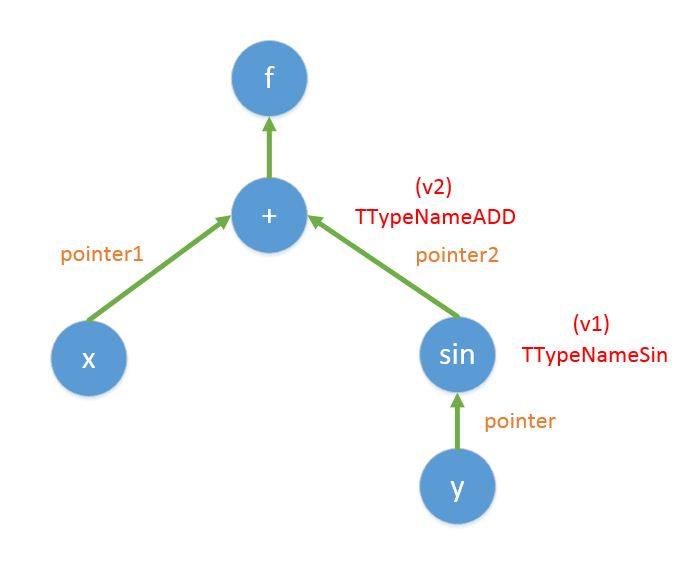
\includegraphics[scale=0.7]{images/DAG1}
	\caption{Directed Acyclic Graph Example}
	%\label{FDD}
\end{figure}
Here are the steps for the AD Taylor mode implementation in the \FADBADpp package.
\begin{itemize}
	\item We initialize x and y of type \texttt{T<double>} and specify the coefficients of the Taylor series for x and y. Thus, the Taylor series of x is $x(t)=1+t+2t^2$ and the Taylor series of y is $y(t)=2+t$.
	\item When processing \texttt{sin(y)}, an object of \texttt{TTypeNameSin<U, N>} type (denoted as $v_1$) will be constructed, which contains a pointer to the single operand y. The 0'th order Taylor-coefficient of v1 will be evaluated.
	\item When we evalute $x+v_1$, an object of \texttt{TTypeNameADD<U, N>} type (denoted as $v_2$) will be constructed, which contains two pointers to operands x and $v_1$ ($v_1$ is of type \texttt{TTypeNameSin<U, N>}). The 0'th order Taylor-coefficient of $v_2$ will be evaluated.
	\item Finally, the result is assigned to variable f. The program calls the overloaded operator ``{\tt =}'' in \fadiff.
	\item If more orders of the Taylor coefficients in f are required, each object like $v_1$ and $v_2$ on the path in the recorded DAG will be re-evaluated to the given order from bottom to top. In the code above, each object in the recorded DAG is re-evaluated to order 10.
\end{itemize}

%\bibliographystyle{siam}
%\bibliography{references}
%\end{document}

% WORK UP TO HERE ---------------------------

% !TEX root = Report.tex

\chapter{Overview of MPFR}\label{ch:mpfr}
MPFR, short for  Multiple Precision Floating-Point Reliable Library, is a portable library written in C for arbitrary precision arithmetic on floating-porint numbers. It is based on the GMP library, aiming to provide a class of floating-point numbers with precise semantics.

We cover a series of basic functions which we use in the multi-precision extension in the \FADBADpp package to be discussed in Chapter \CHref{extension}. For more details regarding the GNU MPFR library, please read the official GNU MPFR manual \cite{MPFRman}.


\section{MPFR library functions}
\subsection{Initialization Functions}
A {\tt mpfr\_t} object must be initialized before storing the first value in it.
\begin{center}
\texttt{void mpfr\_init2 (mpfr\_t x, mpfr\_prec\_t prec)}
\end{center}
initializes x, sets its precision to the default precision, and sets its value to NaN.
\begin{center}
	\texttt{void mpfr\_init (mpfr\_t x)}
\end{center}
initializes x, sets its precision to be exactly \texttt{prec} bits and its value to NaN.
\begin{center}
	\texttt{void mpfr\_clear (mpfr\_t x)}
\end{center}
This function should be called when a {\tt mpfr\_t} variable is not used any more.
\subsection{Arithmetic Functions}
A series of arithmetic functions are given in the MPFR library to process corresponding arithmetic operations for {\tt mpfr\_t} type variables. In these arithmetic functions, a parameter needs to be set for the rounding mode. For example:

\texttt{int mpfr\_add (mpfr\_t rop, mpfr\_t\_op1, mpfr\_t\_op2, mpfr\_rnd\_t rnd)}

gets the addition of two {\tt mpfr\_t} variables and stores the result in the first parameter. Rounding mode needs to be set in the parameter rnd.

\texttt{int mpfr\_sqr (mpfr\_t\_rop, mpfr\_t\_op, mpfr\_rnd\_t rnd)}

\texttt{int mpfr\_sin (mpfr\_t\_rop, mpfr\_t op, mpfr\_rnd\_t rnd)}

Some functions like these two above are used to get the square root or sin value of a {\tt mpfr\_t} variable.

\subsection{Default Precision and Default Rounding Mode}
\subsubsection{Default Precision Setting}
\texttt{void mpfr\_set\_default\_prec (mpfr\_prec\_t prec)}

sets the default precision to be exactly \texttt{prec} bits, where \texttt{prec} can be any integer between \texttt{MPFR\_PREC\_MIN} and \texttt{MPFR\_PREC\_MAX}. The precision of a variable means the number of bits used to store its significand. The default precision is set to 53 bits initially.
\subsubsection{Default Rounding Mode Setting}
\texttt{void mpfr\_set\_default\_rounding\_mode (mpfr\_rnd\_t rnd)}

sets the default rounding mode to \texttt{rnd}, using one of the rounding mode: \texttt{MPFR\_RNDN}, \texttt{MPFR\_RNDZ}, \texttt{MPFR\_RNDU}, \texttt{MPFR\_RNDD},and \texttt{MPFR\_RNDA}. The default rounding mode is to nearest initially.

\section{MPFR C++}\label{sc:mpfrcpp}

Since MPFR library is written in C, it does not support the C++ features like class constructor, destructor and overloaded operators etc. To make it compatible with the AD templates in the FADBAD++ package, a C++ interface or a wrapper for MPFR is required.

MPFR C++ written by Pavel Holoborodko uses a modern C++ design with coverage of classes, templates and function objects. The class wrapping the GNU MPFR library is defined in the header file \texttt{mpreal.h} and named \mpreal, which is to be used in the multiple-precision extension to the FADBAD++ package \cite{mpfrcpp}.


% !TEX root = Report.tex

\chapter{Multi-precision extension in the \FADBADpp package}\label{ch:extension}
In this chapter, we will first discuss how to specialize the templated struct \Op in \fadbad to enable us to use a user-defined class type \texttt{mpreal} instead of built-in C++ type like float and double in the AD templates in the \FADBADpp package. Then we will discuss the problem of temporary objects construction. Finally, we will show how we eliminate temporary objects in this multi-precision extension implementation. 
\section{Specialization of the templated struct \Op in \textbf\texttt{fadbad.h}}\label{sc:opspecwithmpreal}
The template classes in the original \FADBADpp package enable users to differentiate functions that are implemented in built-in C++ types, such as float and double. However, if we want to implement multi-precision in \FADBADpp, we need to use a user-defined class type, say \texttt{mpreal} which supports all the multi-precision operations in the GNU \MPFR library and modern C++ features.

We need to specialize the template \Opn with the class \texttt{mpreal}. The operators used in the general template \Opn like ``{\tt +}'', ``{\tt +=}'', ``{\tt *}'' are all overloaded in the the class \texttt{mpreal}. 

For example, the overloaded operator ``{\tt +=}'' is defined in the class \texttt{mpreal} as
\begin{lstlisting}[numbers=none]
inline mpreal& mpreal::operator+=(const mpreal& v)
{
	mpfr_add(mpfr_ptr(), mpfr_srcptr(), v.mpfr_srcptr(), mpreal::get_default_rnd());
	MPREAL_MSVC_DEBUGVIEW_CODE;
	return *this;
}
\end{lstlisting}
If we have a statement {\tt x+=y}, where x and y are all \mpreal variables, it will call the overloaded operator ``{\tt +=}'' shown above. Since these operators are all overloaded, we could directly use them in the specialized {\tt Op<mpreal>}.

As for elementary functions that have called corresponding elementary functions defined in the C numerics library {\tt math.h} like
\begin{lstlisting}[numbers=none]
static T mySin(const T &x) { return ::sin(x); }
\end{lstlisting}
we could see that \texttt{sin} is also overloaded in the class \texttt{mpreal} as
\begin{lstlisting}[numbers=none]
const mpreal sin(const mpreal& v, mp_rnd_t rnd_mode);
\end{lstlisting}
we could directly use the function \texttt{mpreal::sin} to replace the function {\tt::sin} defined in \texttt{math.h}.
\begin{lstlisting}[numbers=none]
Op<mpreal>::mysin(const mpreal &x) { return mpreal::sin(x); }
\end{lstlisting}
From the example above and based on the specialized templated struct {\tt Op<mpreal>}, we could directly replace built-in C++ types like float and double with the user-defined class {\tt mpreal} in the forward and Taylor mode template class as {\tt F<mpreal> and T<mpreal>}, and accomplish the multi-precision extension in the \FADBADpp package.
\section{Temporary objects issue}
However, we come to another problem, the incessant construction and destruction of temporary objects by using overloaded operators like ``{\tt +}'', ``{\tt -}'', ``{\tt *}'', and ``{\tt /}'', and elementary functions like {\tt mpreal::sin} in \texttt{mpreal} class. For example, consider the following code.
\begin{lstlisting}[numbers=none]
for(unsigned int i=0;i<10;++i)
{
	f = x / Op<T>::mySin(y);
}
\end{lstlisting}	
If the data type of the variables f, x, and y is double, \texttt{Op<double>::mySin(y)} will be called to return a temporary result of type double and divide the double variable x for 10 times. However, if the data type of the variables f, x, and y is of type \texttt{mpreal}, circumstance seems to be more complicated, which involves construction and destruction of temporary objects.

From the \texttt{mpreal.h}, we could see that the declaration for the overloaded operator $/$ is
\begin{lstlisting}[numbers=none]
const mpreal operator/(const mpreal& a, const mpreal& b);
\end{lstlisting}
\texttt{Op<mpreal>::mySin(y)} is called to return a temporary object of class \texttt{mpreal}. Then, this temporary object divides x and from the declaration above, the division will return another temporary object of class \texttt{mpreal} too, which will be assigned to the variable f. According to the C++ mechanism, a temporary object of a class will be constructed first and at the end of the statement, the temporary object will be destructed \cite{C++Primer}. Although it is a very neat way, these construction and destruction procedures will be iteratively executed 10 times. Hence, we would like to come up with a way to avoid unnecessary temporary objects from being constructed especially those in the loops or nested loops, which will be a severe performance hit.
 

\section{Temporary objects elimination}
In this section, we discuss how to avoid temporary objects in the loops from being generated.
\subsection{Improving the specialized templated struct {\tt Op<mpreal>} in \textbf\texttt{fadbad.h}}
In Section \SCref{opspecwithmpreal}, we used overloaded elementary functions defined in {\tt mpreal.h} to replace elementary functions defined in the C numerics library {\tt math.h}. But they will return temporary objects of the type {\tt mpreal}. Hence, we will discuss how to amend these functions to avoid returning temporary objects.
\subsubsection{Adding Operation functions to replace direct use of overloaded operators defined in \textbf\texttt{mpreal.h}}
First, we consider the use of overloaded operators ``{\tt +}'', ``{\tt -}'', ``{\tt *}'', and ``{\tt /}''. Suppose we have the statement
$$x + y$$
where x and y are all of type {\tt mpreal}. It will call the overloaded operator ``{\tt +}'' defined in {\tt mpreal.h}. The declaration of the overloaded operator ``{\tt +}'' defined in {\tt mpreal.h} is
\begin{lstlisting}[numbers=none]
const mpreal operator+(const mpreal& a, const mpreal& b)
\end{lstlisting}
It will always return a temporary variable of type \mpreal. Noticing that the declaration of the add operation function defined in the MPFR library is
\begin{lstlisting}[numbers=none]
int mpfr_add (mpfr_t rop , mpfr_t op1 , mpfr_t op2 , mpfr_rnd_t rnd )
\end{lstlisting}


The result is not returned as an object, but stored in the object the first parameter \texttt{rop} points to. Hence, this function does not return a temporary object of type \mpreal. Using this kind of arithmetic operation functions defined in the MPFR library directly will be an alternative way to replace the use of overloaded operators ``{\tt +}'', ``{\tt -}'', ``{\tt *}'', and ``{\tt /}'' defined in {\tt mpreal.h}.

Here, we will add some functions for addition, subtraction, multiplication, and division in the specialized templated struct {\tt Op<mpreal>}, which will be used to replace the use of overloaded operators ``{\tt +}'', ``{\tt -}'', ``{\tt *}'', and ``{\tt /}'' defined in {\tt mpreal.h}.
For example, the definition for the addition function in {\tt Op<mpreal>} to replace the use of overloaded operator ``{\tt +}'' is
\begin{lstlisting}[numbers=none]
  static void mpreal_add(mpreal &rop, const mpreal &op1, const double &op2, mpfr_rnd_t rnd = DEFAULT_RNDM)
  {
  	if (rop.get_prec() != DEFAULT_PREC)
  	rop.set_prec(DEFAULT_PREC, DEFAULT_RNDM);
  	mpfr_add_d(rop.mpfr_ptr(), op1.mpfr_ptr(), op2, rnd);
  }
\end{lstlisting}

The result is returned through a pointer \texttt{rop} as the first parameter in this function instead of being returned as an object to avoid temporary objects from being generated. Inside the function, function {\tt mpf\_add\_d} is directly called to process the addition. Similar to other overloaded operators ``{\tt -}'', ``{\tt *}'', and ``{\tt /}'', we will add functions into {\tt Op<mpreal>} to process subtraction, multiplication and division without returning temporary objects.
\subsubsection{Improving specialized elementary functions}
We need to consider the use of the overloaded elementary functions defined in {\tt mpreal.h}, which will return temporary objects of type \mpreal. For example, the declaration of the overloaded \texttt{sin} function defined in {\tt mpreal.h} is
\begin{lstlisting}[numbers=none]
const mpreal sin(const mpreal& v, mp_rnd_t rnd_mode);
\end{lstlisting}
It will return the result as a temporary object of type \mpreal. Similar to the operator ``{\tt +}'', we could find a function in the MPFR library to have the same functionality.
\begin{lstlisting}[numbers=none]
int mpfr_sin (mpfr_t rop , mpfr_t op , mpfr_rnd_t rnd)
\end{lstlisting}
The result here is returned through the pointer \texttt{rop} as the first parameter. In this way does this function avoid temporary objects from being generated. Then, we replace all the overloaded elementary functions occurring in the specialized templated struct {\tt Op<mpreal>} with functions that have the same functionality defined in the MPFR library. For example,
\begin{lstlisting}[numbers=none]
Op<mpreal>::mysin(const mpreal &x) { return mpreal::sin(x); }
\end{lstlisting}
is amended to
\begin{lstlisting}[numbers=none]
  static void mpreal_sin(mpreal &rop, const mpreal &x, mpfr_rnd_t rnd = DEFAULT_RNDM)
  {
  if (rop.get_prec() != DEFAULT_PREC)
  rop.set_prec(DEFAULT_PREC, DEFAULT_RNDM);
  mpfr_sin(rop.mpfr_ptr(), x.mpfr_ptr(), rnd);
  }
\end{lstlisting}
Similarly, we replace the functions such as {\tt cos}, {\tt tan}, {\tt exp}, {\tt log}, using the functions defined in the MPFR library directly.

So far, all the functions in the specialized templated struct {\tt Op<mpreal>} do not return results as temporary objects.
\subsection{Temporary objects elimination method in \textbf\texttt{fadiff.h}}
We modify every templated elementary function in \fadiff.
\begin{itemize}
	\item As for all the templated elementary functions in \fadiff, we need to give a specialization for our user-defined data type \mpreal. Hence, when calling the functions with parameters of type \mpreal, the specialized elementary functions will be called instead of the general one. For example, the original declaration of the general templated \texttt{sin} function is
\begin{lstlisting}[numbers=none]
template <typename T>
inline FTypeName<T, 0> sin(const FTypeName<T, 0>& a)
\end{lstlisting}
	We need to specialize this general template to our user-defined data type {\tt mpreal}. Then, the declaration becomes as
\begin{lstlisting}[numbers=none]
inline FTypeName<mpreal, 0> sin(const FTypeName<mpreal, 0>& a)
\end{lstlisting}	
	\item We replace the arithmetic operators ``{\tt +}'',``{\tt -}'', ``{\tt *}'', and ``{\tt /}'' and functions defined in the struct \texttt{Op<T>} with elementary functions defined in the specialized struct \texttt{Op<mpreal>} step by step and keep the precedence of all the operands in the statements. For example, suppose we have
	
	%{\textbf{In the Original sin function in fadiff.h}}
	%\lstinputlisting[firstline=1980,lastline=1991]{\INCDIR/fadiff.h}
	\begin{center}
		{\tt a+b*Op<T>::sin(c)} 
	\end{center}
	In this statement, two main points should be paied attention to.
	\begin{itemize}
		\item Functions defined in \texttt{Op<T>} should be replaced with corresponding elementary functions defined in \texttt{Op<mpreal>}.
		\item We should avoid the use of arithmetic operators ``{\tt +}'',``{\tt -}'', ``{\tt *}'', and ``{\tt /}'' and replace them with the corresponding elementary functions defined in the struct {\tt Op<mpreal>}. Meanwhile, we need to focus on the right precedence for all the operands.\\
	\end{itemize}
	After the modification, this statement is rewritten as
\begin{lstlisting}[numbers=none]
Op<mpreal>::mpreal_sin(TEMP_RESULT, c);
Op<mpreal>::mpreal_mul(TEMP_RESULT1, b, TEMP_RESULT);
OP<mpreal>::mpreal_add(TEMP_RESULT, a, TEMP_RESULT);
\end{lstlisting}
	To store indispensable temporary results among the calculations, we need to create several static variables of type \mpreal in advance. Empirically, two will be sufficient in our implementation. {\tt TEMP\_RESULT} and {\tt TEMP\_RESULT1} are two static variables of type \mpreal defined in advance in the struct {\tt Op<mpreal>}. By keeping the right precedence for all the operands and modifying the original statement step by step, {\tt TEMP\_RESULT} is the final result.
	%\lstinputlisting[firstline=1993,lastline=2005]{\INCDIR/fadiff.h} 
\end{itemize}
\subsection{Temporary objects elimination method in \textbf\texttt{tadiff.h}}
In tadiff.h, two main places will be modified.
\begin{enumerate}
	\item  We modify every arithmetic class in \tadiff like {\tt TTypeNameSIN} and {\tt TTypeNameEXP}.
	\begin{itemize}
		\item We specialize all the general arithmetic class templates like {\tt TTypeNameEXP<T, N>} with our user-defined data type mpreal. For example, The original declaration of our general arithmetic  class {\tt TTypeNamEXP} is
\begin{lstlisting}[numbers=none]
template <typename U, int N>
struct TTypeNameEXP : public UnTTypeNameHV<U, N>
\end{lstlisting}
		Then we need to specialize this general template with our user-defined data type \mpreal. After the modification, the declaration of the specialized form is
\begin{lstlisting}[numbers=none]
template <int N>
struct TTypeNameEXP : public UnTTypeNameHV<mpreal, N>
\end{lstlisting}
		\item In the virtual function \texttt{eval} defined in every class like \texttt{TTypeNameMUL<mpreal, N>, TTypeNamePOW<mpreal,N>} etc, similar to the modification in \fadiff, we replace operators such as $+, -, *, /$ and elementary functions defined in the struct \texttt{Op<T>} with corresponding functions from struct \texttt{Op<mpreal>}. For example, suppose we have this statement in the virtual function {\tt eval} in the class \texttt{TTypeNameEXP<mpreal,N>}.
\begin{lstlisting}[numbers=none]
Op<U>::mycadd(a, (Op<U>::myOne() - Op<U>::myInteger(j)}/ Op<U>::myInteger(i)) * b * c);
\end{lstlisting}
	%{\textbf{In the Original Exp class (eval function)}}
	%\lstinputlisting[firstline=1860,lastline=1876]{\INCDIR/tadiff.h} 
	Here is the precedence for all the operands in this statement.
	\begin{itemize}
	
		\item \texttt{temp\_result1 = Op<U>::myInteger(j) / Op<U>::myInteger(i);}
		\item \texttt{temp\_result2 = Op<U>::myOne() - temp\_result1;}
		\item \texttt{temp\_result3 = temp\_result2 * b;}
		\item \texttt{temp\_result4 = temp\_result3 * c;}
		\item \texttt{a += tmep\_result4;}
	\end{itemize}
		Then, We replace all the arithmetic operators and functions defined in \texttt{Op<U>} with elementary functions defined in the specialized \texttt{Op<mpreal>}. Here is the modification for each step.
	\begin{itemize}
		\item \texttt{TEMP\_RESULT1 = (double)j/(double)i;}
		\item \texttt{Op<mpreal>::mpreal\_sub(TEMP\_RESULT2, 1, TEMP\_RESULT1);}
		\item \texttt{Op<mpreal>::mpreal\_mul(TEMP\_RESUL3, TEMP\_RESULT2, b);}
		\item \texttt{Op<mpreal>::mpreal\_mul(TEMP\_RESULT4, TEMP\_RESUL3, c);}
		\item \texttt{Op<mpreal>::myCadd(a, TEMP\_RESULT4);}
	\end{itemize}
	Since no more than two temporary results are used in the same function, we only need two static \mpreal objects defined in advance in the struct \texttt{Op<mpreal>}. Thus, the final version of the modification is\\\
\begin{lstlisting}[numbers=none]
TEMP_RESULT1 = (double)j/(double)i
Op<mpreal>::mpreal_sub(TEMP_RESULT, 1, TEMP_RESULT1)
Op<mpreal>::mpreal_mul(TEMP_RESUL1, TEMP_RESULT, b)
Op<mpreal>::mpreal_mul(TEMP_RESULT, TEMP_RESUL1, c)
Op<mpreal>::myCadd(a, TEMP_RESULT)
\end{lstlisting}
	where {\tt TEMP\_RESULT} and {\tt TEMP\_RESULT1} are static variables of data type \mpreal defined in advance in the templated struct {\tt Op<mpreal>}.
	%{\textbf{In the Specialized Exp class (eval function)}}
	%\lstinputlisting[firstline=1889,lastline=1910]{\INCDIR/tadiff.h}
	\end{itemize}
	\item We modify overloaded arithmetic operation functions (such as operator ``{\tt +}'', ``{\tt -}'', ``{\tt *}'', ``{\tt /}'' and {\tt sin}, {\tt cos}, {\tt exp} and so on) in tadiff.h.
	
	\begin{itemize}
		\item As for all the template elementary functions in \fadiff, we need to give a specialization to our user-defined data type {\tt mpreal}. Hence, when calling the functions with parameters of type {\tt mpreal}, the specialized arithmetic operation functions will be called instead of the general ones. For example, the original declaration of the general arithmetic operation function template is
\begin{lstlisting}[numbers=none]
template <typename U, int N>
TTypeName<U, N> exp(const TTypeName<U, N>& val)
\end{lstlisting}	
	Then, We specialize this general form to our user defined data type {\tt mpreal} as
\begin{lstlisting}[numbers=none]
template <int N>
TTypeName<mpreal, N> exp(const TTypeName<mpreal, N>& val)
\end{lstlisting}	
		\item In these arithmetic operation functions in tadiff.h, any arithmetic operators or elementary functions defined within \texttt{Op<U>} used to evaluate the first item in Taylor expansions should be replaced with corresponding functions defined in \texttt{Op<mpreal>}. Temporary results from the evaluation should be stored first in the static \mpreal objects defined in the specialized struct \texttt{Op<mpreal>} before passed into a constructor. For example, suppose we have the following statement in {\tt exp}
\begin{lstlisting}[numbers=none]
new TTypeNameEXP<U, N>(Op<U>:: myExp(a));
\end{lstlisting}			
		where \texttt{a} is a variable of data type U.
		
		This statement is modified in the specialized function for our use-defined data type \mpreal as
\begin{lstlisting}[numbers=none]
Op<mpreal>::mpreal_exp(TEMP_RESULT, a);
new TTypeNameExp<mpreal, N>(TEMP_RESULT);
\end{lstlisting}		
		where {\tt TEMP\_RESULT} is a static variable of data type \mpreal defined in advance in the templated struct {\tt Op<mpreal>}.
		%\lstinputlisting[firstline=1917,lastline=1924]{\INCDIR/tadiff.h} 
		%\textbf{The overloaded exp function after the modification.}
		%\lstinputlisting[firstline=1926,lastline=1940]{\INCDIR/tadiff.h} 
	\end{itemize}
\end{enumerate}
% !TEX root = Report.tex

\chapter{Examples}\label{ch:examples}
In this chapter, two examples are given to show how to use the multi-precision extension feature in the forward mode and Taylor mode templates in the modified FADBAD++ package. In each example, the max norm between the double datatype and the mpreal datatype is used to check the difference to verify the correctness of our modification of the original FADBAD++ package. 
%In the end, the last example is to show an application of using modified Taylor series mode template to solve an ordinary differential equation(ODE).
\newpage
\section{The heap-form template in the forward method}
{\textbf{We modified ExampleFAD2.cpp from the distribution of FADBAD++ as follows.}}\\
\lstinputlisting{\SRCDIR/ExampleFAD2.cpp}
\newpage
First of all, to use the templates defined in the namespace fadbad, we need to declare \texttt{using namespace fadbad}. Then, we need to set the default working precision and the default rounding mode for all the mpreal variables by using the two library functions in the GNU MPFR library below

\texttt{void mpfr\_set\_default\_prec (mpfr\_prec\_t prec)}

\texttt{void mpfr\_set\_default\_rounding\_mode (mpfr\_rnd\_t rnd)}

In this version, we use the heap-form forward method template to define all the variables. We use mpreal whose working precision is 128 bits and double whose precision is 53 bits to calculate the final result in the function \texttt{func}. Finally, we check the difference using the max norm between mpreal and double to verify the correctness of the modification. The output is
\lstinputlisting{\OUTDIR/ExampleFAD2_result.txt}
\newpage
\section{The Taylor-expansion method template }
{\textbf{In ExampleTAD1.cpp}}
\lstinputlisting{\SRCDIR/ExampleTAD1.cpp}
\newpage
The equation to compute in this example is defined below:
$$f(x(t),y(t))=\sin(x(t) + y(t) / 3.2 - \cos(5.263))$$
in which all the variables are of \texttt{T<U>} type. The arithmetic operation functions will now "record" a directed acyclic graph (DAG) while computing the function value (which is the 0'th order Taylor-coefficient) \cite{IntroAl}. \\
The recorded DAG for this equation is
\begin{figure}[H]
	\centering
	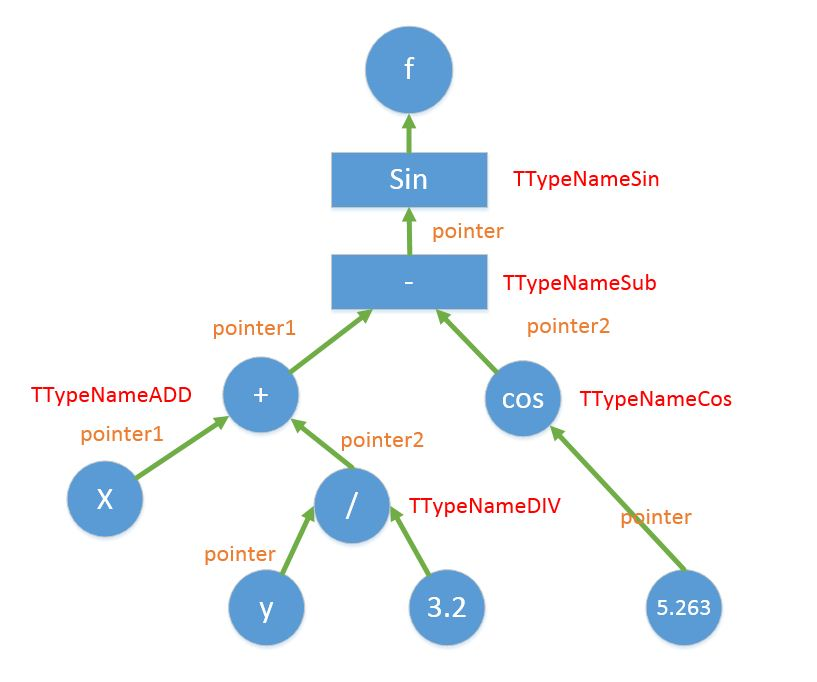
\includegraphics[scale=0.55]{images/DAG2}
	\caption{Directed Acyclic Graph in ExampleTAD1}
	%\label{FDD}
\end{figure}
Finally, we check the difference using the max norm between mpreal and double to verify the correctness of the modification. The output is
\newpage
\lstinputlisting{\OUTDIR/ExampleTAD1_result.txt}
%\section{An application using the Tadiff to solve an ODE}
%{\textbf{In ExampleTAD2.cpp}}
%\lstinputlisting{\SRCDIR/ExampleTAD2.cpp}
%In this example, we use the Taylor-expansion template to solve an ODE which is a possible applicaton for the Taylor-expansion template. The recorded DAG connecting two instance variables in the class TODE is simple below:
%\begin{figure}[H]
%	\centering
%	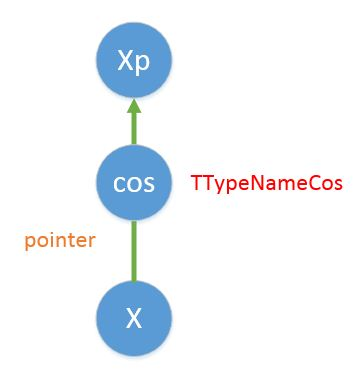
\includegraphics[scale=0.5]{images/DAG3}
%	\caption{DAG in class TODE}
%\end{figure}
%The output is shown below:
%\lstinputlisting{\OUTDIR/ExampleTAD2_result.txt}
\newpage
\section{Makefile}
The overall makefile to make all the example executives is shown below:
\lstinputlisting{\SRCDIR/makefile}
%\appendix
\chapter{Appendix}
\section{Proposed design}
In this section we show the detailed ER diagram of our proposed design. The ER diagram has been split into four different figures for better readability. We have also discussed the new tables that were created to improve customer relationship management.
\begin{figure}
\centering
\includegraphics[height=11cm,width=15cm]{images/trans1}
\caption{Purchase Tables}
\label{Pdesign1}
\end{figure}
\begin{figure}
\centering
\includegraphics[height=11cm,width=15cm]{images/profile_tables1}
\caption{Profile Tables}
\label{Pdesign2}
\end{figure}
\begin{figure}
\centering
\includegraphics[height=10cm,width=16cm]{images/summary1}
\caption{Summary Tables}
\label{Pdesign3}
\end{figure}
\begin{figure}
\centering
\includegraphics[height=10cm,width=14cm]{images/survey1}
\caption{Survey Tables}
\label{Pdesign4}
\end{figure}
\subsection{New Tables Schemas}
\textbf{Vendor: }The client related information are stored in this table.\\
\textbf{Vendor\_visit: }In this table, the \emph{user\_id} attribute records the customer information and the \emph{vendor\_id} attribute records the corresponding client information he/she visited.\\
\textbf{User\_product\_interaction: }This table captures the customer information and the corresponding product information he/she had shown interest on. A record is inserted into the table every time a customer interacts with a product. The attribute \emph{start\_time} captures the time when an interaction begins and the attribute \emph{end\_time} captures the time when the interaction ends. We can use the time difference (end\_time - start\_time) to extract the level of interest of a customer on a particular product (the higher the time difference, then higher the customer's interest on the product).\\
\textbf{Customer\_purchases: }This table contains the customer information (such as customer's id) and the corresponding product information he/she purchased (product id, amount spent on the product). This table also contains the date and time of each purchase. A record is inserted into the table every time a customer purchases a product.\\
\textbf{Product\_groups: }Products are classified into groups and a unique \emph{group\_id} is assigned to each group. \emph{Product\_groups} table combined with \emph{Customer\_purchases} table enables the organization to market other products in the group based on the customer purchase pattern. For example, the electronics group contain products such as phones, laptops and tablets. If a customer had purchased a phone (information extracted from the transactions table) the organization can  market laptops and tablets to the same customer (as laptops and tablets belongs to the same electronics group).\\\\
The Summary tables contain aggregated information extracted from the above mentioned tables. This enhances the analysis process (e.g., total sales of a product, most profitable customer), as  the organization need not combine multiple tables or run analytical functions (such as sum, difference and total count) to extract information. They can execute a selection query on the summary tables to extract the above mentioned highlights. \texttt{Figure \ref{Pdesign3}.User\_summary} for each customer contains, the total products purchased, the number of clients he/she visited and the total time he/she spent on a product. \texttt{Figure \ref{Pdesign3}.Vendor\_event\_summary} for each client contains, total sales, total time spent by the customers and the number of customers that visited. \texttt{Figure \ref{Pdesign3}.Product\_summary} for each product contains, total quantity sold, the number of clients interacted and total time spent by the customers. The products are classified into groups and \texttt{Figure \ref{Pdesign3}.Group\_summary} for each group contains, total time and amount spent by the customers.
\newpage
\section{Implemented Queries}
{\Large\textbf{SALES QUERIES}\par}
\begin{lstlisting}
--1) Total sales across all events
SELECT name AS event_name,SUM(amount) AS Total_event_sales
FROM transactions,event
GROUP BY name;


--2) Total sales across all clients for one event
SELECT name AS event_name,name AS clients_name,transaction_date,SUM(amount) AS total_amount
FROM transactions,event,client
WHERE event id = '957'
GROUP BY name,transaction date;


--3) Client and Customer details for products purchased at an event
SELECT id,product_name,name AS clients_name,name AS event_name,first_name
FROM product_transactions,products,clients,customer
WHERE product_id IN
(SELECT product_id
FROM  product_transactions, transactions
WHERE event_id = '957'
GROUP BY product_id, clients_id)
AND id = '957';


--4) Identify the top-5 sold products (in terms of quantity sold) at a given event.  Return the product id and name for each product.
SELECT id, product_name
FROM product
WHERE id IN
(SELECT product_id
FROM  product_transactions,transactions
WHERE event_id = '957'
GROUP BY product_id
ORDER BY count(product_id) DESC
FETCH FIRST 5 ROWS ONLY);
\end{lstlisting}
{\Large \textbf{CUSTOMER QUERIES}}
\begin{lstlisting}
--5) For each customer-to-product interaction at a given client, return the customer's product rating and the customer feedback.
SELECT DISTINCT question, answer, customer_id
FROM survey answers,questions,answers
WHERE question_id BETWEEN 49 AND 109 AND customer_id IN
(SELECT customer_id
FROM customer_product_interaction
WHERE  Clients_id = 1 );


--6) Return the top-5 products according to men (measured by their interaction time).
SELECT id, product_name
FROM product
WHERE id IN
(SELECT product_id
FROM customer_product_interaction,survey_answers
WHERE question_id = '33' AND answer_id = '39'GROUP BY
product_id ORDER BY
COUNT(product_id) DESC
FETCH FIRST 5 ROWS ONLY;


--7) ROI per client across all events
SELECT DISTINCT id, first_name, Clients_id, name AS Clients_name, SUM(amount) AS transaction sum
FROM ps_behavior_profile_500K,customer,clients
WHERE transaction_id IS NOT NULL AND customer_id IN
(SELECT customer_id
FROM transactions t)
GROUP BY id, first_name, Clients_id, name
ORDER BY transaction sum DESC;


--8) Identify all products interacted and later purchased by a given customer
SELECT id AS ProdID Interacted, prod_name AS ProdName Interacted,id AS ProdID purchased, prod_name AS ProdName Purchased
FROM (SELECT DISTINCT product_id AS id, product_name AS prod_name FROM customer_product_interaction,product
WHERE customer_id = 232 AND product_id NOT IN
(SELECT product_id FROM transactions,product_transactions
WHERE customer_id = 232)) temp1
,(SELECT DISTINCT product_id AS id, p1.product_name AS prod_name  FROM customer_product_interaction, product
WHERE customer_id = 232 AND product_id IN
(SELECT product_id FROM transactions,product_transactions
WHERE customer_id = 232)) temp2;
\end{lstlisting}
{\Large\textbf{AGGREGATION QUERIES}}
\begin{lstlisting}
--9) For each potential customer, return client name and product name he/she expressed interest
SELECT id,first_name,last_name,name AS Clients_name,product_name,Time_spent_product
FROM customer_product_interaction,product,clients
WHERE product_id = id AND id IN
(SELECT customer_id
FROM customer_product_interaction
WHERE NOT EXISTS
(SELECT 'X'
FROM transactions
WHERE customer_id = customer_id ));
\end{lstlisting}
{\Large\textbf{OVERLAPPING QUERY GROUPS}}\\
\noindent\rule{12.2cm}{0.4pt}\\
{\large\textbf{SALES AGGREGATION QUERIES}}\\\\
The following two queries return most popular products in terms of customer interaction time. Query 10A) runs over warehouse data and Query 10B) runs over transactional data. We compare the running time of both the queries.
\begin{lstlisting}

--10A)
SELECT product_id, product_name AS product_name, SUM(Time_spent_product)
FROM behavior_profile,product
GROUP BY product_id, product_name
ORDER BY SUM(Time_spent_product) DESC;


--10B)
SELECT product_id, product_name AS product_name, SUM(Time spent_Product)
FROM customer_product_interaction,product
GROUP BY product_id,product_name
ORDER BY SUM(Time_spent_Product) DESC;
\end{lstlisting}
{\large\textbf{CUSTOMER AGGREGATION QUERIES}}\\\\
The following two queries return client name and product name each potential customer expressed interest on. Query 11A) runs over warehouse data and Query 11B) runs over transactional data. We compare the running time of both the queries.
\begin{lstlisting}
--11A)
SELECT id, first_name, last_name, email, name AS Clients_name, product_name, Time_spent_product
FROM product,Clients
AND id IN
(SELECT customer_id
FROM behavior_profile
WHERE NOT EXISTS
(SELECT 'X'
FROM transactions
WHERE customer_id = customer_id));


--11B)
SELECT id, first_name, last_name, email, name AS Clients_name, product_name, Time_spent_Product
FROM product,Clients
AND id IN
(SELECT customer_id
FROM customer_product_interaction
WHERE NOT EXISTS
(SELECT 'X'
FROM transactions
WHERE customer_id = customer_id));
\end{lstlisting}
{\large\textbf{COMPARATIVE QUERIES }}
\begin{lstlisting}
--12) Top 5 products across all clients
Original design
select distinct t2.PRODUCT_NAME as pname ,t1.product_id as pid, count(t1.product_id) as Quantity from rogers_check_in t1
inner join rogers_product_list t2 on t1.product_id = t2.id
group by t1.product_id,t2.PRODUCT_NAME
union all
select distinct t3.PRODUCT_NAME as spname ,t4.product_id as spid, count(t4.product_id) as SQuantity from samsung_tap_history t4
inner join samsung_product_list t3 on t4.product_id = t3.id
group by t4.product_id,t3.PRODUCT_NAME
order by Quantity desc
fetch first 5 rows only;

Proposed design
select distinct t2.PRODUCT_NAME,t1.product_id, count(product_id) as quantity from n_user_product_interaction t1
inner join n_product_list t2 on t1.product_id = t2.id
group by t1.product_id,t2.PRODUCT_NAME
order by quantity desc
fetch first 5 rows only;


--13) Uniquely identify customers across all clients and the products they have expressed their interest
Original design
select distinct t1.user_id,t1.first_name,t1.last_name from rogers_user_profile t1
where t1.user_id not in
(select user_id from rogers_check_in t2)
union all
select distinct t1.user_id,t1.first_name,t1.last_name from samsung_user_profile t1
where t1.user_id not in
(select user_id from samsung_tap_history t2);

Proposed design
select distinct t1.id,t1.first_name,t1.last_name from n_user t1
where t1.id not in
(select user_id from n_user_product_interaction t2);


--14) Uniquely identify customers across all clients who want to be notified by clients (Whether customers want clients to contact them)
Original design
select * from rogers_user_profile where contact_consent = 1;

Proposed design
select * from n_user
where id in
(select user_id from n_vendor_visit where contact_consent = 1);


--15) Uniquely identify the survey responses for a given customer across all clients
Original design
select t2.question,t3.answer from rogers_survey_data t1
inner join rogers_questions t2 on t1.question_id = t2.id
inner join rogers_answers t3 on t1.answer_id = t3.id
where user_id in
(select user_id from rogers_user_profile where first_name = 'Ethan' and last_name = 'Do' fetch first row only)
union all
select t2.question,t3.answer from samsung_survey_data t1
inner join samsung_questions t2 on t1.question_id = t2.id
inner join samsung_answers t3 on t1.answer_id = t3.id
where user_id in
(select user_id from samsung_user_profile where first_name = 'Ethan' and last_name = 'Do'fetch first row only);

Proposed design
select t2.question,t3.answer from n_survey_answers t1
inner join n_questions t2 on t1.question_id = t2.id
inner join n_answers t3 on t1.answer_id = t3.id
where user_id in
(select id from n_user where  first_name = 'Ethan' and last_name = 'Do');


--16) Uniquely identify customers who applied for a smart card across all clients
Original design
select id from
(select id from samsung_nfc_list
union all
select id from rogers_nfc_list);

Proposed design
select id from n_nfc_list;

\end{lstlisting} 
% add other chapters go here. don't forget to reset the counters each time!
\bibliographystyle{siam}
\bibliography{references}
\label{NumDocumentPages}
\end{document}

